%% Neural Networks For Classification
%% 2014/07/10
%% by Soren Goyal
%%-----------------------------------------------------------------------------------------------------
\documentclass[journal,transmag]{IEEEtran}

\usepackage{cite}
\usepackage[cmex10]{amsmath}
\usepackage{amssymb}
\usepackage{algorithm}
\usepackage{algpseudocode}

%\usepackage{algorithmicx}

\usepackage{array}
\usepackage{graphicx}
	%\graphicspath{images/}
\usepackage{url}

\begin{document}

\title{CSE 5243\\Homework 2}
\author{\IEEEauthorblockN{Soren Goyal, Ohio State University}}

%\IEEEtitleabstractindextext{
%\begin{abstract}
%Recognition of objects using Deep Neural Networks is an active area of research and many breakthroughs have been made in the last few years. The paper attempts to indicate how far this field has progressed. The paper briefly describes the history of research in Neural Networks and describe several of the recent advances in this field. The performances of recently developed Neural Network Algorithm over benchmark datasets have been tabulated. Finally, some the applications of this field have been provided.
%\end{abstract}
% Note that keywords are not normally used for peer review papers.
%\begin{IEEEkeywords}
%Convolutional, Neural Networks, Datasets, ILSVRC, Pooling, Activation Functions, Regularization, Object Recognition, Datasets
%\end{IEEEkeywords}}

% make the title area
\maketitle
\section{Section 1: Introduction}
	The Income dataset is extracted from 1994 US Census database. The data base contains 520 records. Each record in the database represents a person. The records hold a number of personal details about the people such as Marital Status, Occupation, Education Level, etc. All the attributes are described in full length in Table \ref{table:database-description}. The records are classified into two sets -``people with income greater than \$50K" and "people with income less than or equal to \$50K". The ``$<=$50K" class contains 420 records while the ``$>$50K" class has the remaining 100. The exploratory analysis was concerned with answering two main questions - 
\begin{itemize}
\item There are 16 attributes for each person. What are the characteristics of each attribute ? Both qualitative and statistical ? What values are missing ? 
\item The records are classified into either of the two categories ``$>$50K" and ``$<=$50K". What are the attributes that best determine the classification category and what are attributes that don't seem to have any effect?
\end{itemize}

Table: II tabulates the occurrence of missing values in the database.

\begin{table}[h]
\label{table:database-description}
\caption{Description of the Data Attributes}
\centering
	\begin{tabular}{| c | m{140 pt} |}
		\hline
		Attribute Name & Description\\
		\hline
		ID & Unique identifier of each record. Takes integer values and ranges from 15 to 32378.\\
		\hline
		age & Age of the person in years. It ranges from 15 to 82.\\
		\hline
		workclass & Type of employer. It has 5 categories - Federal-gov, Private, Self-emp-inc, Self-emp-not-inc and State-gov. \\
		\hline
		fnlwgt & No description available. \\
		\hline
		\hline
		education & Education level of the person. It is divided into 16 levels - Preschool, 1st-4th, 5th-6th, 7th-8th, 9th, 10th, 11th, 12th, HS-grad, Some-college, Assoc-voc, Assoc-acdm, Bachelors, Masters, Prof-school, Doctorate.\\
		education\_cat & Each education level is assigned a numerical value. It starts at $1$ for Preschool and goes upto $16$ for a Doctorate.\\
		\hline
		marital\_status & It takes six different Divorced, Married-AF-spouse, Married-spouse-absent, Never-married, Separated and Widowed.\\
		\hline
		occupation & It has 13 levels - Adm-clerical, Craft-repair, Exec-managerial, Farming-fishing, Handlers-cleaners, Machine-op-inspct, Other-service, Priv-house-serv, Prof-specialty, Protective-serv, Sales, Tech-support and Transport-moving. It also has missing values labeled as ``?".\\
		\hline
		relationship & It is unknown as to which relationship does this refer to. It takes six possible values - Husband, Not-in-family, Other-relative, Own-child, Unmarried and Wife.\\
		\hline
		race & It takes four possible values Amer-Indian-Eskimo, Asian-Pac-Islander, Black, Other and White. \\
		\hline
		gender & It is either Male or Female.\\
		\hline
		capital\_gain & It takes a continuous value from 0 to 99999. $91\%$ of the persons have a 0 in this field.\\
		\hline
		capital\_loss & It too takes a continuous value from 0 to 4356. $96\%$ of the people also have a 0 in this field. \\
		\hline
		hour\_per\_week & It refers to the number of hours a person works in a week. It ranges from 2 hours to 99 hours.\\
		\hline
		native\_country & The country of origin. This attribute can take over 25 values. However, 90\% of the times it takes "United States".\\
		\hline
		class & There are two classes labeled using strings - ``$<=$50K" and ``$>$50K".\\
		\hline
	\end{tabular}
\end{table}

\begin{table}[h]
\label{table:missing-values}
\caption{Missing Values in the Dataset}
\centering
	\begin{tabular}{| c | c |}
		\hline
		Attribute Name & Missing Values/Total number of Records\\
		\hline
		ID & $0$\\
		\hline
		age & $0$\\
		\hline
		workclass & $0.054$ \\
		\hline
		fnlwgt & $0$ \\
		\hline
		education & $0$\\
		\hline
		education\_cat & $0$\\
		\hline
		marital\_status & $0$\\
		\hline
		occupation & $0.054$ \\
		\hline
		relationship & $0$ \\
		\hline
		race & $0$ \\
		\hline
		gender & $0$ \\
		\hline
		capital\_gain & $0$ \\
		\hline
		capital\_loss & $0$ \\
		\hline
		hour\_per\_week & $0$\\
		\hline
		native\_country & $0.12$\\
		\hline
		class & $0$ \\
		\hline
	\end{tabular}
\end{table}

%%%%%%%%%%%%%%%%%%%%%%%%%%%%%%%%%%%%%%%%%%%%%%%%%%%%%%%%%%%%%%%%%%%%%%%%%%%%%%%%
\subsection{Characteristics of Attributes}
The Income dataset has 16 attributes, out which two don't contribute to the understanding of data. The \emph{ID} attribute is a number unique to each record and hence does not have any useful underlying pattern. The meaning of \emph{fnlwgt} could not be discerned and so it was not analyzed further. The remaining attributes were analyzed and the following peculiarities were found - 
\begin{itemize}
	\item \emph{Age (Fig:1)}- The age of the people in the higher income bracket ranged from 25 to 79 years. The majority of the people were in the range of 36 to 52 years. The age in the lower income bracket had a different distribution. It was more spread out. The ages ranged from 17 to 82 years. The majority of the people were relatively younger in this income bracket with the 50\% of the people lying between 25 and 45 years. Although there is a considerable overlap, the peaks of the distributions are distinguishable. The mean of higher income bracket is at 45 while the peak of lower income bracket is at 36.78 years, 10 years less.
		\begin{figure}[h]
			\label{fig:age-hist}
			\caption{Histogram of Age for both the classes}
			\centering
			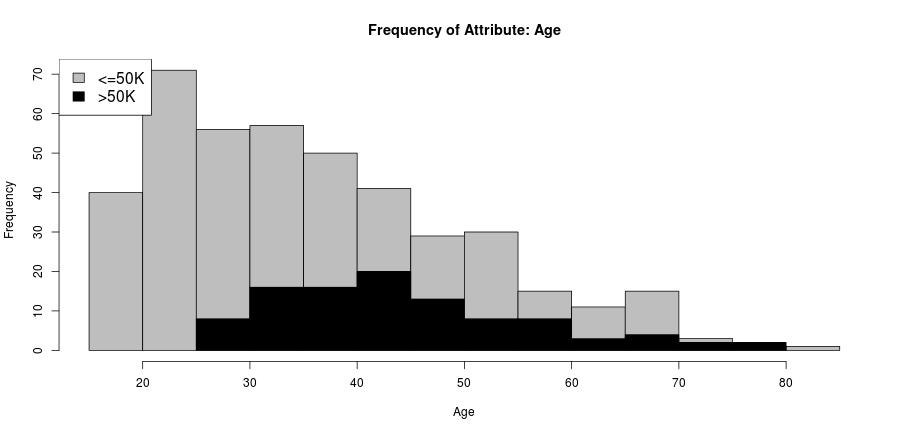
\includegraphics[width=0.5\textwidth]{images/age-hist.jpg}
		\end{figure}
	\item \emph{Capital Gain (Fig:2)} - Out of the 420 people in lower income bracket only 3\% made positive capital gains, while nearly 73\% of the 100 in the upper income bracket made capital. Also the capital gains of the upper income bracket are significantly more.
		\begin{figure}[h]
			\label{fig:capital-gain-hist}
			\caption{Histogram of Capital Gains for both the classes}
			\centering
			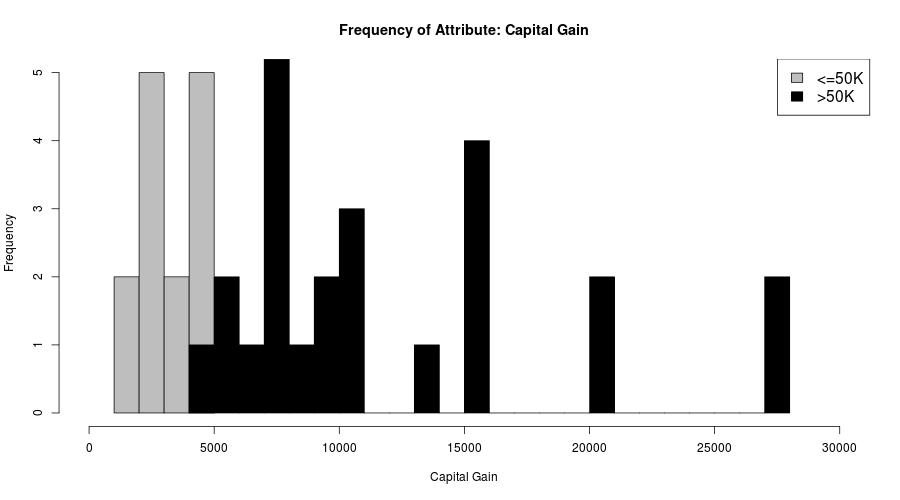
\includegraphics[width=0.5\textwidth]{images/capital_gain-hist.jpg}
		\end{figure}
	\item \emph{Capital Losses (Fig:3)} - Most of the people did not make any capital losses. Only 3\% of people in both the classes suffered a capital loss. But since the number of lower income bracket is significantly higher, we can conclude that a person suffering a capital loss has a higher probability of being in the lower income bracket.
		\begin{figure}[h]
			\label{fig:capital-loss-hist}
			\caption{Histogram of Capital Losses for both the classes}
			\centering
			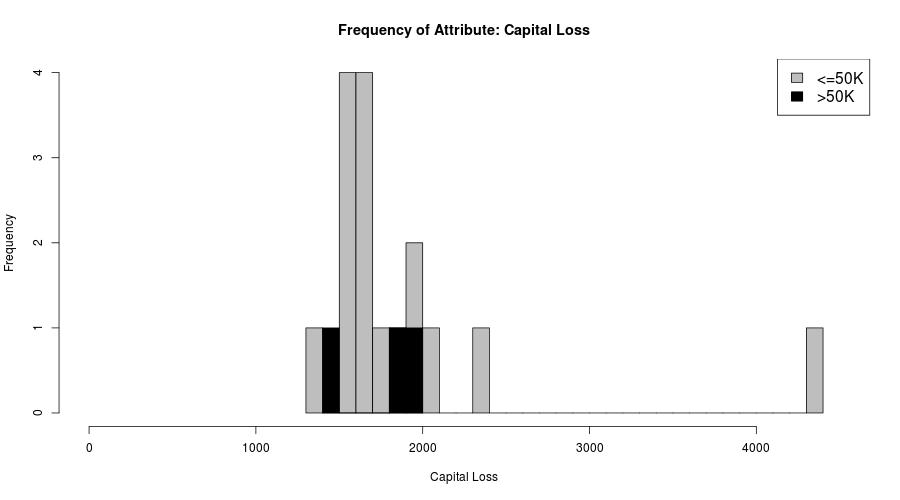
\includegraphics[width=0.5\textwidth]{images/capital_loss-hist.jpg}
		\end{figure}
	\item \emph{Education (Fig:4)} - All education categories have mix of people from upper and lower income groups. However, certain education levels have a greater proportion of people having income more than \$50K. If a person comes from the following groups - preschool, $5^{th}$ - $6^{th}$, $7^{th} - 8^{th}$, $11^{th}$, $12^{th}$ or Masters then their is a greater than 50\% chance that they belong to the upper income bracket. Also it is interesting to note that 86\% of all the people have a maximum education degree of HS-grad, Some-college or Bachelors.
		 \begin{figure}[h]
			\label{fig:education-bar}
			\caption{Barplot showing the number of people vs education category}
			\centering
			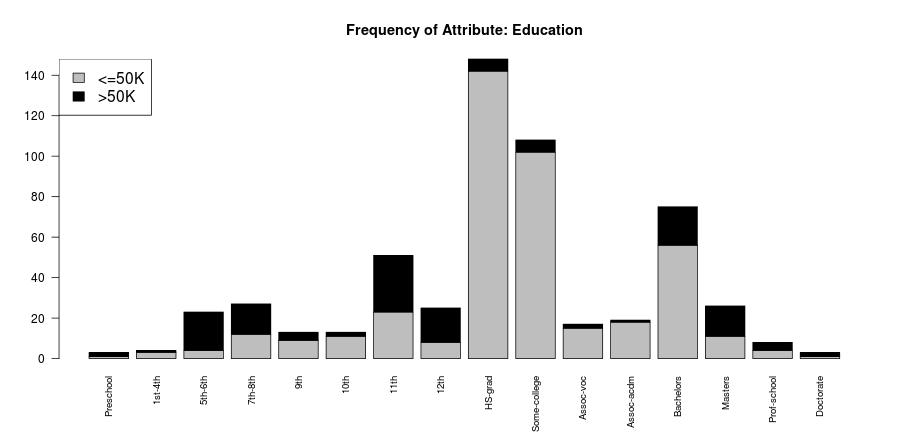
\includegraphics[width=0.5\textwidth]{images/education-bar.jpg}
		\end{figure}
	\item \emph{Marital Status (Fig:5)} -75\% people in the higher income bracket are married. This is also the single largest marital status in the higher income bracket. The single largest category in the lower income bracket is Never-Married. Nearly 45\% of the people  in lower income bracket have never married.
		 \begin{figure}[h]
			\label{fig:marital-status-bar}
			\caption{Barplot showing the number of people plotted against their Marital Status}
			\centering
			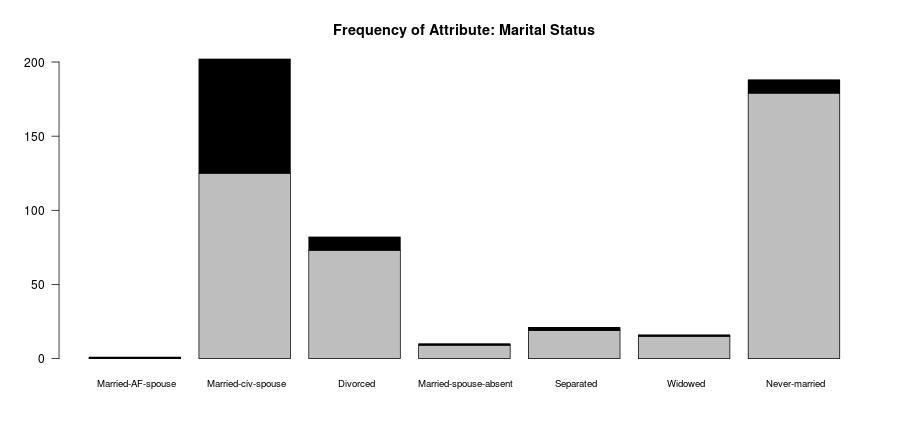
\includegraphics[width=0.5\textwidth]{images/marital-status-bar.jpg}
		\end{figure}
	\item \emph{Native Country (Fig:6)} - For most of the people in the higher income bracket the country of origin is USA. A large number of people in lower income bracket too belong to USA. This brings the ratio of higher to lower income for USA down to 0.22. This ratio is 1 for three countries - France, Italy and Japan. For 16 out of the 26 countries the ratio is 0.
		 \begin{figure}[h]
			\label{fig:native-country}
			\caption{Ratio of people in '>50K' to total people grouped by Native Country}
			\centering
			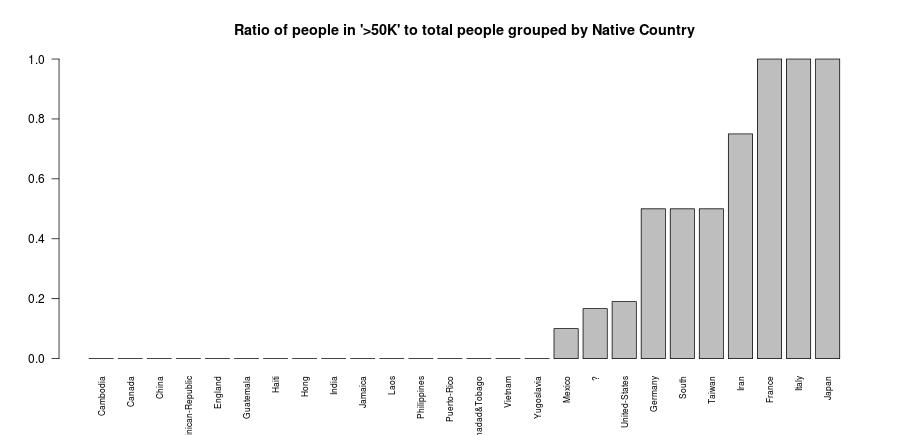
\includegraphics[width=0.5\textwidth]{images/native-country.jpg}
		\end{figure}
	\item \emph{Occupation (Fig:7)} - Occupations requiring professional knowledge or managerial knowledge have most of the upper income people. However, the ratio of upper income people never goes above 0.5 for any occupation. This makes this attribute difficult to be used for any discrimination. The people in other-services and Private house service always belong to the Lower income category.
		 \begin{figure}[h]
			\label{fig:occupation-bar}
			\caption{Ratio of people in Upper Income Bracket grouped by Occupation}
			\centering
			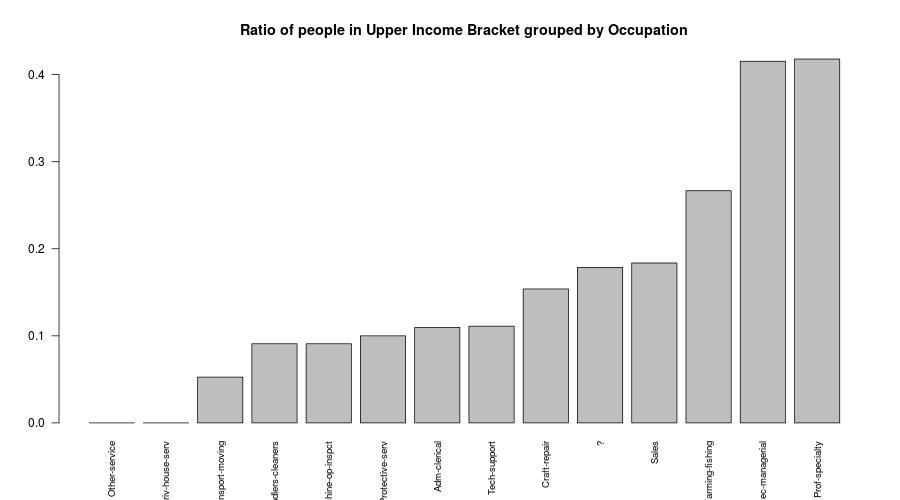
\includegraphics[width=0.5\textwidth]{images/occupation-bar.jpg}
		\end{figure}
	\item \emph{Hours Per Week (Fig:8)} - Overall most people work for moderate number of hours per week,  i.e - ranging from 25 to 45 hours. In the upper income category almost everyone works in this range. The distrbution for lower income people is a bit more spreadout.
		 \begin{figure}[h]
			\label{fig:hour-per-week-hist}
			\caption{Hours worked per week for both the categories}
			\centering
			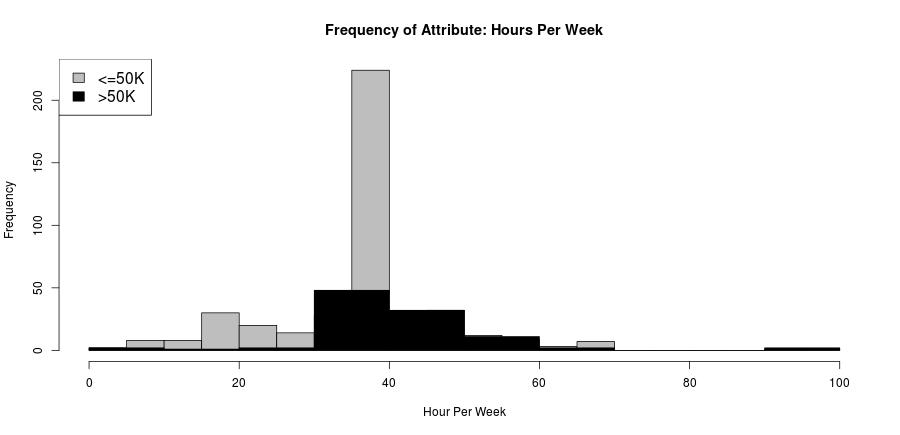
\includegraphics[width=0.5\textwidth]{images/hours-hist.jpg}
		\end{figure}
\end{itemize}
%%%%%%%%%%%%%%%%%%%%%%%%%%%%%%%%%%%%%%%%%%%%%%%%%%%%%%%%%%%%%%%%%%%%%%%%%%%%%%%%
\subsection{Patterns in Plots}
A scatter plot (Fig:9)  between the education, hours per week, capital gain and capital loss offers some interesting insights. The people with lower educational qualifications tend to have higher capital gains. Most people with a capital gain tend to be in the higher income category while people with capital loss tend to be in the lower income category. People who have capital gains mostly work moderate number of hours per week. People below High School Grad level of education work for relatively lesser hours per week, as compared to people with college education or higher. The number of working hours of people in between these two, span from the very low to very high.\\
\begin{figure}[h]
			\label{fig:scatter-matrix}
			\caption{Matrix of Scatter Plots}
			\centering
			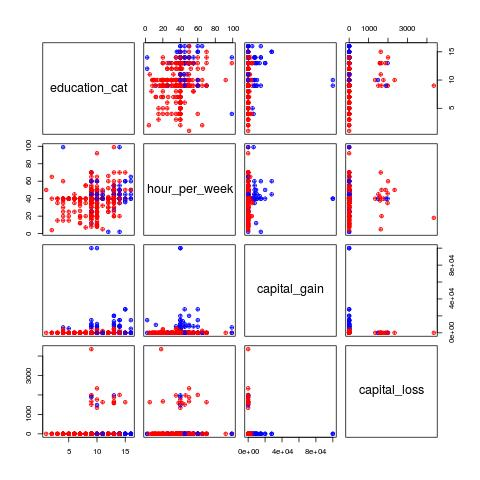
\includegraphics[width=0.5\textwidth]{images/scatter-matrix.jpg}
\end{figure}
Certain attributes can be used to discriminate between the classes. In this cursory analysis the two classes tend to separate out a lot when a scatter plot is plotted between Capital Gain education and hours worked per week. This scatter plot shows two distinct clusters of high income category. The first one is made no capital gains has high education and moderate working hours. The other cluster made significant capital gains and hence stands out.\\
 \begin{figure}[h]
			\label{fig:3d-scatter}
			\caption{3D Scatter plot of the attributes Capital Gain, Capital Loss and Hours Worked with points colored to differentiate the class}
			\centering
			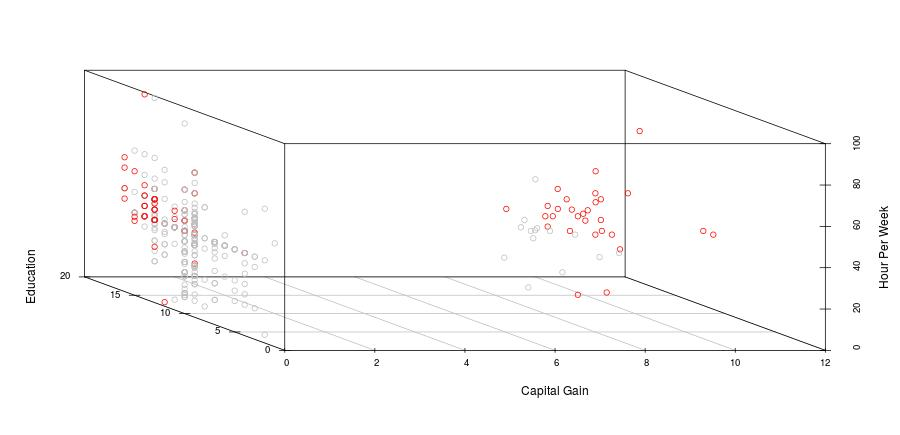
\includegraphics[width=0.5\textwidth]{images/3d-scatter.jpg}
	\end{figure}
To better understand the nature of clusters in the dataset, an analysis using Nearest Neighbor computation is required which is done in section 3.\\
%%%%%%%%%%%%%%%%%%%%%%%%%%%%%%%%%%%%%%%%%%%%%%%%%%%%%%%%%%%%%%%%%%%%%%%%%%%%%%%%


\section{Section 2: Evaluation of performance}
	
The variations mentioned in the previous section were tried and the analysis of the perfromance of KNN classifier is presented in this section.
\subsection{Classifier Performance for Iris Dataset}
	\textbf{Classifier 1}
	\begin{itemize}
		\item Preprocessing - Simple Scaling
		\item Proximity Metric - Euclidean Distance
		\item Voting - Inverse Distance Weighted Voting
	\end{itemize}
	The confusion matrix for k = 5 is given in Fig: ?
	\begin{figure}[h]
		\label{fig:iris_k=5}
		\caption{Confusion Matrix k = 5 (Datset:Iris Classifier:1)}
		\centering
		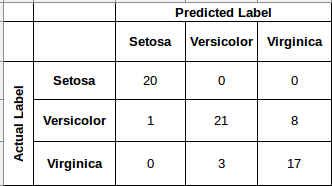
\includegraphics[width=0.4\textwidth]{images/iris_k=5.png}
	\end{figure}
	From the analysis in the previous assignment, we know that the setosa class was distinctly separated from the other two classes. The effect of this can be seen in the confusion matrix. The KNN classifier was able to classify all instances of setosa correctly. Also, there was only 1 false positive for setosa. On the other hand, versicolor and virginica had significant overlap. The algorithm did a good job on them too. Although, roughly 33\% of Versicolor were falsely classified as Virginica. Overall the accuracy of this classfier was 82\% \\
	
	\textbf{Classifier 2}
	\begin{itemize}
		\item Preprocessing - Simple Scaling (same as before)
		\item Proximity Metric - Cosine Similarity
		\item Voting - Inverse Distance Weighted Voting (same as before)
	\end{itemize}
	The confusion matrix for $k = 5$ is given in Fig: ??.
	\begin{figure}[h]
		\label{fig:iris_consine_k=5}
		\caption{Confusion Matrix k = 5 (Datset:Iris Classifier:2)}
		\centering
		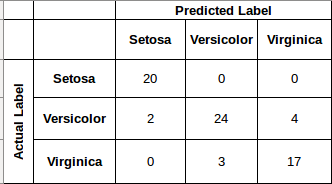
\includegraphics[width=0.4\textwidth]{images/iris_cosine_k=5.png}
	\end{figure}
	This classifier performed better than the previous one. The accuracy increased to 87\%, by simply by using cosine similarity instead of euclidean similarity. Here to setosa was much more easily distinguised as compared to the other two classes, although the false positives in setosa increased increased by small amount.\\

\subsection{Classifier Performance for Income Dataset}
For binary income dataset, the classifier had to be optimized over two parameters had to be optimized - the number of nearest neighbours $k$ and threshold for making the prediction. \\
To optimum $k$ for the classifier would be the $k$ for which the ``Area Under the Roc Curve" is maximized. To find the optimum $k$, the roc graphs were computed over the test set for $k$'s ranging from 1 to 100. It was expected that the area would increase with $k$, peak and then plateau out. The $k$ at the peak would then be optimum.\\
For a picking the optmium threshold, we maximized the accuracy of the classifier. To determine the highest accuracy, the threshold was varied keeping the $k$ was fixed. The threshold for which the accuracy is maximum was taken to be the optimum threshold.

\textbf{Classifier 1}
	\begin{itemize}
		\item Preprocessing - Simple Scaling
		\item Proximity Metric - Euclidean Distance
		\item Voting - Inverse Distance Weighted Voting
	\end{itemize}
	For this classifier the Area under ROC reaches maximum at $k = 38$. In Fig. ?? four ROC curves have been plotted. The ROC curve for $k=38$ has the most area underneath it, although it is surpassed at few points by other ROC curves. The accuracy for $k=38$ is plotted as a function of $threshold$. It increase monotonically as $threshold$ increases and is maximum for $threshold=1$ (point not on the curve). This is beacuse of the highly skewed class ratio, the highest accuracy is obtained when all records are classified as negative. This is clearly not a $threshold$ to pick. However, if we give more weightage to true positives, the Accuracy Vs Threshold Curve might for values less than one, giving a more reasonable classifier. \\
	\begin{figure}[h]
		\label{fig:classifier1_auc}
		\caption{Plot of Area Under the Roc curve for different values of k for Income Classifier 1. Maxima is achieved at k = 38}
		\centering
		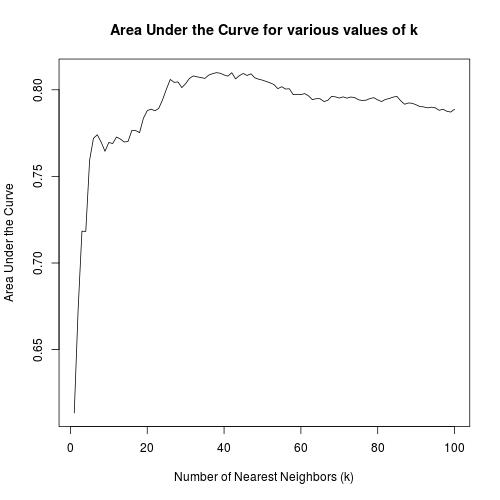
\includegraphics[width=0.3\textwidth]{images/income_classifier1/auc.jpg}
	\end{figure}	
	\begin{figure}
		\label{fig:classifier1_roc}
		\caption{ROC curves for different values of k for Income Classifier 1}
		\centering
		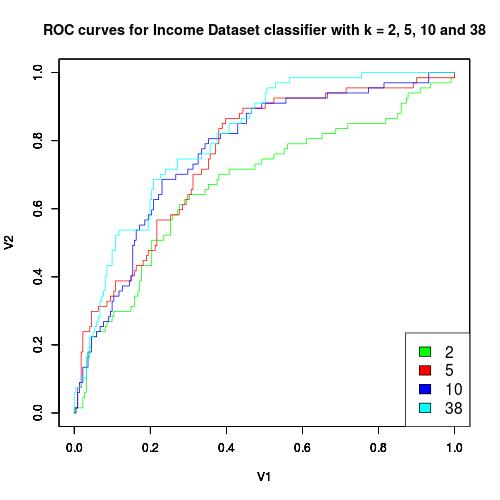
\includegraphics[width=0.3\textwidth]{images/income_classifier1/roc.jpg}
	\end{figure}
	\begin{figure}
		\label{fig:classifier1_accuracy}
		\caption{Plot of Accuracy Vs Threshold Values for k = 38}
		\centering
		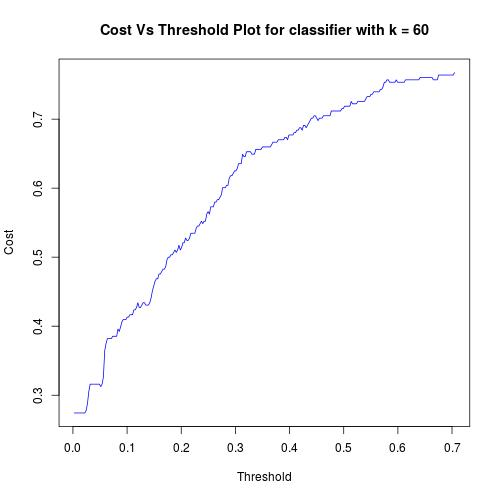
\includegraphics[width=0.3\textwidth]{images/income_classifier1/accuracy.jpg}
	\end{figure}	
	
\textbf{Classifier 2}
	\begin{itemize}
		\item Preprocessing - Simple Scaling
		\item Proximity Metric - Cosine Similarity
		\item Voting - Inverse Distance Weighted Voting
	\end{itemize}
	The Iris dataset should a good improvement when the proximity metric was changed from eulidean distance to cosine similarity. However, the same is not observed in income dataset. For this classifier the ``area under the curve" reaches its maximum at k=38. Fig. ?? contains the plot for the AUC. Four different ROCs have been plotted in Fig. ??. The trend in AUC and ROC is similar to what was observed in previous classifier. The best accuracy too is obtained for $threshold=1$. The false positive rate increase way to fast in comparison to the true positive rate.\\
	\begin{figure}[h]
		\label{fig:classifier2_auc}
		\caption{Plot of Area Under the Roc curve for different values of k for Income Classifier 2. Maxima is achieved at k = 36}
		\centering
		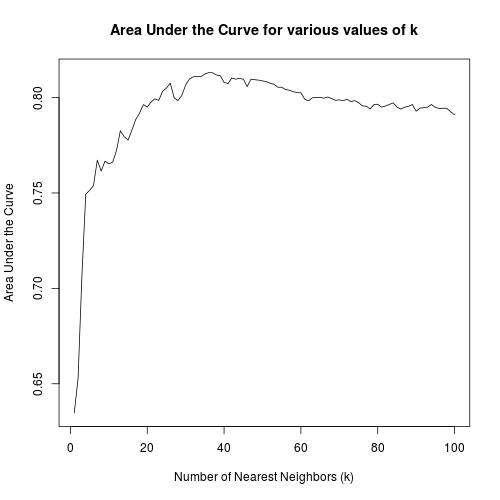
\includegraphics[width=0.3\textwidth]{images/income_classifier2/auc.jpg}
	\end{figure}	
	\begin{figure}
		\label{fig:classifier2_roc}
		\caption{ROC curves for different values of k for Income Classifier 2}
		\centering
		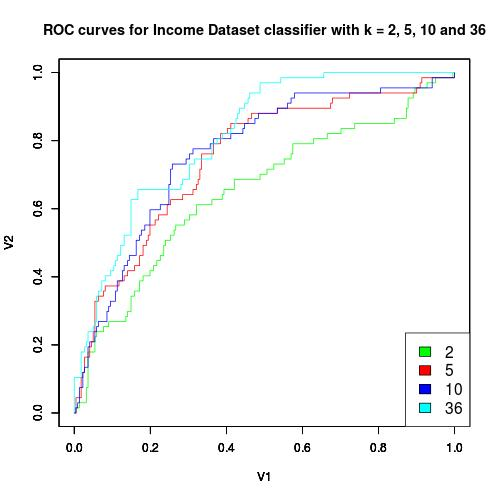
\includegraphics[width=0.3\textwidth]{images/income_classifier2/roc.jpg}
	\end{figure}
	\begin{figure}
		\label{fig:classifier2_accuracy}
		\caption{Plot of Accuracy Vs Threshold Values for k = 36}
		\centering
		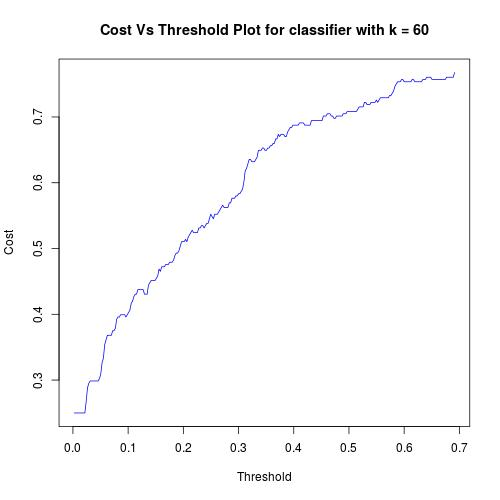
\includegraphics[width=0.3\textwidth]{images/income_classifier2/accuracy.jpg}
	\end{figure}
	
\textbf{Classifier 3} - Best Performance
	\begin{itemize}
		\item Preprocessing - Simple Scaling with Binning
		\item Proximity Metric - Cosine Similarity
		\item Voting - Inverse Distance Weighted Voting
	\end{itemize}
	Based on the previous performance of the previous two classfiers, it was felt that the attributes should be preprocessed such that the similar record have similar values. In that spirit, many categories were merged. For e.g - There were 26 native countries, with 12 having only one record. Each of these records belonged to the same class. The records would be 1 unit apart if simple dissimilarity is computed. But for this classifier all these records were bunched together in a single category and hence bringing them closer.\\
	These preprocessing did have a small postive effect. The maximum area under the curve incrased by 5\% (Fig. ??). The ROC for optimium $k$ also reaches a saturation at lower FPR as compared to Classfier 1 or 2. However, the the optimium $threshold$ is still $1.0$.\\
	\begin{figure}[h]
		\label{fig:classifier3_auc}
		\caption{Plot of Area Under the Roc curve for different values of k for Income Classifier 3. Accuracy keeps increaing beyond hundred}
		\centering
		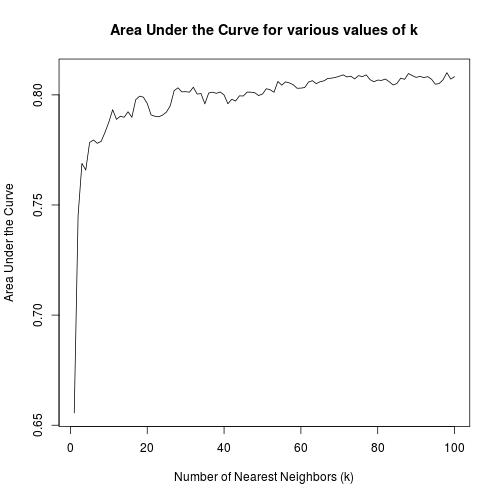
\includegraphics[width=0.3\textwidth]{images/income_classifier3/auc.jpg}
	\end{figure}	
	\begin{figure}
		\label{fig:classifier1_roc}
		\caption{ROC curves for different values of k for Income Classifier 3}
		\centering
		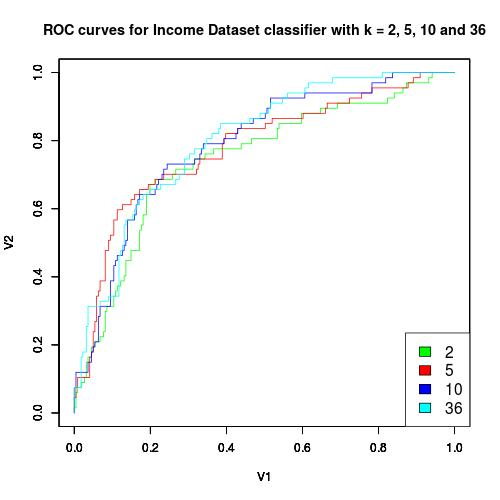
\includegraphics[width=0.3\textwidth]{images/income_classifier3/roc.jpg}
	\end{figure}
	\begin{figure}
		\label{fig:classifier3_accuracy}
		\caption{Plot of Accuracy Vs Threshold Values for k = 40}
		\centering
		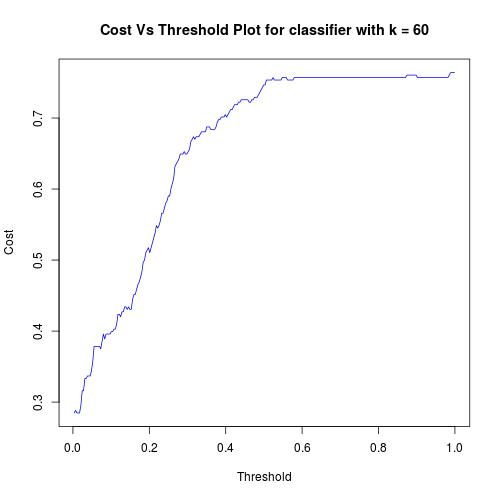
\includegraphics[width=0.3\textwidth]{images/income_classifier3/accuracy.jpg}
	\end{figure}
	
\subsection{Answer to Select Homework Questions}
A,B) The Precision, Recall and F-Measure  are plotted in Fig. ??\\
\begin{figure}
	\label{fig:confusion}
	\caption{Precision, Recall and F-Measure for Classifier 3 of Income Data test set}
	\centering
	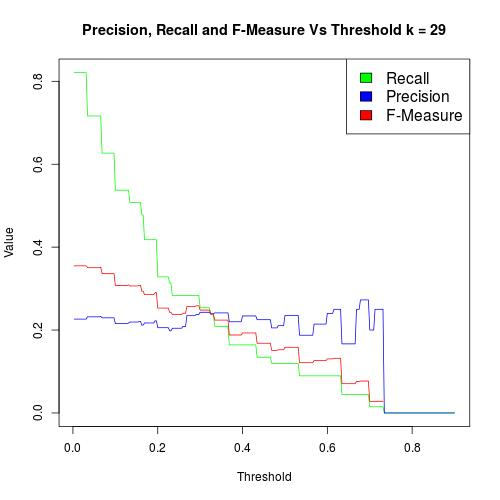
\includegraphics[width=0.3\textwidth]{images/prf.jpg}
\end{figure}
D) There was effect of proximity measure. It was more pronuced on Iris than Income dataset.\\
E) To understand the effect of $k$ on the classifier the AUC can be observed. As mentioned earlier in this report the classfier becomes better for a while, then it peaks and then plateaus. (Fig. ??)\\
F) The third varion in Section. ?? was added becuase the algorithm was not working well with data.

\section{Section 3: Comparision with Off-the-Shelf kNN}
	\subsection{Off-The-Shelf kNN on Income Dataset}
	\begin{figure}[h]
		\label{fig:classifier2_auc}
		\caption{Plot of Area Under the Roc curve for different values of k for Income Classifier 2. Maxima is achieved at k = 36}
		\centering
		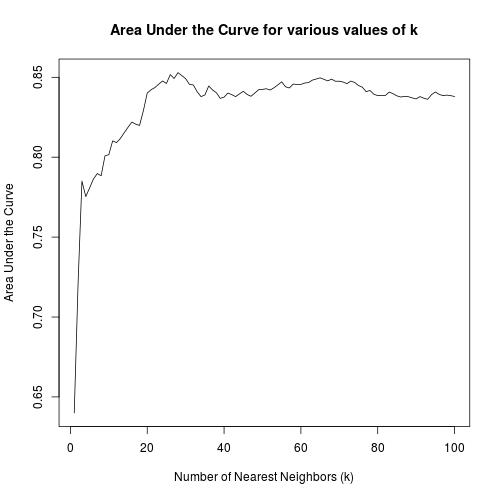
\includegraphics[width=0.3\textwidth]{images/native-knn/auc.jpg}
	\end{figure}	
	\begin{figure}
		\label{fig:classifier2_roc}
		\caption{ROC curves for different values of k for Income Classifier 2}
		\centering
		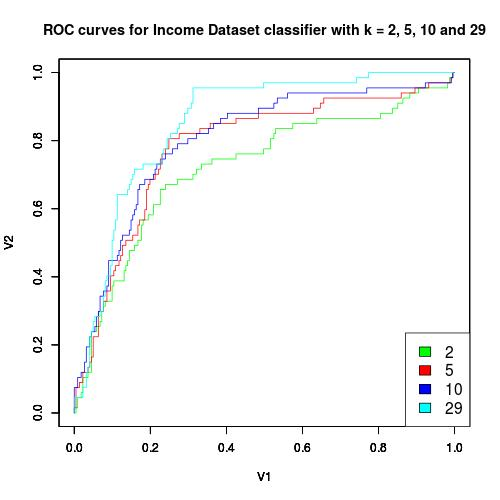
\includegraphics[width=0.3\textwidth]{images/native-knn/roc.jpg}
	\end{figure}
	\begin{figure}
		\label{fig:classifier2_accuracy}
		\caption{Plot of Accuracy Vs Threshold Values for k = 36}
		\centering
		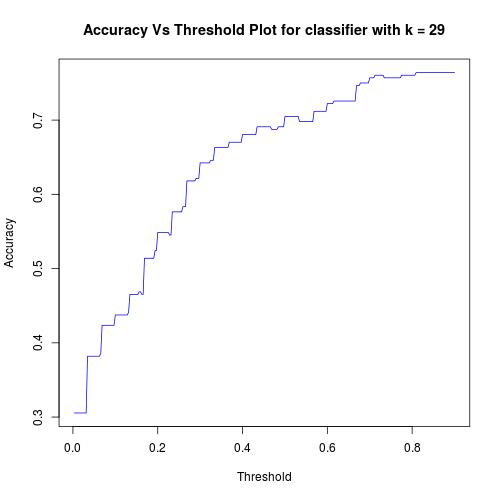
\includegraphics[width=0.3\textwidth]{images/native-knn/accuracy.jpg}
	\end{figure}
	



\end{document}


